\section{Исследование функций и уравнений задачи}
1. Пусть $x^2-10x+q=0.$ При каких $q$ сумма квадратов корней данного уравнения равна 2?\\
2. Пусть $x^2-6x+q=0.$ При каких $q$ сумма квадратов корней данного уравнения равна 4?\\
3. Сколько решений может иметь система $\begin{cases} ax+y+b=0,\\ (x-c)^2+y^2=4.\end{cases}?$\\
4. Сколько решений может иметь система $\begin{cases} kx+y+l=0,\\ (x+c)^2+y^2=4.\end{cases}?$\\
5. Найти область определения функции $f(x)=\sqrt{\cfrac{x(x^2+x-12)(x^2-3x+2)}{(x^2-x-6)(-x+5)}}.$\\
6. Найти область определения функции $f(x)=\sqrt{\cfrac{-x(x^2-2x-15)(x^2-6x+8)}{(x^2-11x+30)(x+1)}}.$\\
7. При каком $a$ один из корней уравнения $x^2-\cfrac{15}{4}x+a^3=0$ будет квадратом другого?\\
8. При каком $a$ один из корней уравнения $x^2-\cfrac{63}{4}x+a^3=0$ будет квадратом другого?\\
9. Найти область определения функции $y(x)=\cfrac{1}{(x-2)\sqrt{4+3x-x^2}}.$\\
10. Найти область определения функции $y(x)=\cfrac{3}{(x-1)\sqrt{3+2x-x^2}}.$\\
11. При каких $k$ модуль разности корней уравнения $x^2-kx+15=0$ равен 2?\\
12. При каких $k$ модуль разности корней уравнения $x^2-kx+3=0$ равен 2?\\
13. При каких $k$ уравнение $kx^2-(k+1)x+2k-1=0$ имеет два различных корня?\\
14. При каких $k$ уравнение $kx^2-(k-1)x+2k+1=0$ имеет два различных корня?\\
15. Найдите наибольшее значение функции $y=-x+2\sqrt{x}-2.$\\
16. Найдите наибольшее значение функции $y=-x+4\sqrt{x}-5.$\\
17. Найдите функцию $f(x),$ если $f(2x-3)=4x-5.$\\
18. Найдите функцию $f(x),$ если $f(2x+3)=4x+5.$\\
19. При каких значениях $a$ уравнение $2ax^2+(10-a)x-a+5=0$ имеет ровно один корень?\\
20. При каких значениях $a$ уравнение $2ax^2+(10+a)x-a-5=0$ имеет ровно один корень?\\
21. Не решая уравнения $2x^2-3x-11=0,$ найдите $\cfrac{x_2}{1+x_1}+\cfrac{x_1}{1+x_2},$ где $x_1$ и $x_2$ его корни.\\
22. Не решая уравнения $9x^2+18x-8=0,$ найдите $x_1^3+x_2^3,$ где $x_1$ и $x_2$ его корни.\\
23. Найдите все значения параметра $a,$ при которых корни уравнения $(a^2-1)x^2+(2a+1)x-3=0$ лежат по разные стороны от точки $x_0=1.$\\
24. Найдите все значения параметра $b,$ при которых число $(-1)$ заключено между корнями уравнения $(4-b^2)x^2-(3b-1)x+7=0.$\\
25. Найти $a,$ если $f(x)=x^2-6x+a$ и её наименьшее значение равно 1.\\
26. Найти $a,$ если $f(x)=-x^2+4x+a$ и её наибольшее значение равно 2.\\
27. При каких $a$ множество решений неравенства $(a-3)x^2-(a+1)x+a+1\geqslant0$ является отрезком?\\
28. При каких $a$ множество решений неравенства $(a+2)x^2-(a-1)x+a-1\geqslant0$ является отрезком?\\
29. Найти наибольшее и наименьшее значения выражения $m^2-\cfrac{4}{n},$ если $-3\leqslant m\leqslant-\cfrac{\sqrt{2}}{2},\ 1,6\leqslant n\leqslant 2.$\\
30. Найти наибольшее и наименьшее значение выражения $b-0,4a^2,$ если $-5\leqslant a\leqslant-1,5,$\\$-0,5\leqslant b\leqslant2,4.$\\
31. Найдите все значения параметра $a,$ при которых число $2$ заключено между корнями уравнения $x^2+(a-5)x+a^2-a=0.$\\
32. Найдите все значения параметра $a,$ при которых число $(-1)$ заключено между корнями уравнения $x^2-(a-7)x+a^2-6a=0.$\\
33. Высота над землёй подброшенного вверх мяча меняется по закону $h(t)=1,6+13t-5t^2,$ где $h$ --- высота в метрах, $t$ --- время в секундах, прошедшее с момента броска. Сколько секунд мяч будет находиться на высоте не менее 4 метров?\\
34. Высота над землёй подброшенного вверх мяча меняется по закону $h(t)=1,4+9t-5t^2,$ где $h$ --- высота в метрах, $t$ --- время в секундах, прошедшее с момента броска. Сколько секунд мяч будет находиться на высоте не менее 3 метров?\\
35. При каких значениях параметра $a$ корни уравнения $ax^2+(a^2+5a-2)x+a+4=0$ расположены симметрично относительно точки $x_0=-2?$\\
36. При каких значениях параметра $a$ корни уравнения $ax^2+(a^2+a-2)x+a+4=0$ расположены симметрично относительно точки $x_0=-1?$\\
37. Найдите наименьшее значение функции $y=7+\sqrt{x^2-2x+5}.$\\
38. Найдите наименьшее значение функции $y=6+\sqrt{3-x^2-2x}.$\\
39. Найдите все значения параметра $a,$ при которых уравнение $ax^2+(4a+2)x+3a+1,5=0$ имеет единственный корень.\\
40. Найдите все значения параметра $a,$ при которых уравнение $ax^2-(2a+6)x+3a+3=0$ имеет единственный корень.\\
41. Найдите наименьшее значение выражения $23-\cfrac{16}{x^2-2x+5}.$\\
42. Найдите наибольшее значение выражения $5+\cfrac{16}{x^2+2x+5}.$\\
43. Найдите наибольшее значение выражения $x^2-4xy+y^2,$ если $x-y=3.$\\
44. Найдите наибольшее значение выражения $5x^2+4xy-5y^2,$ если $2x-y=1.$\\
45. При каких значениях $a$ уравнение $x^3+6x^2+ax=0$ имеет два различных корня?\\
46. При каких значениях $a$ уравнение $4x^3+4x^2+ax=0$ имеет два различных корня?\\
47. Найдите значение выражения $\sqrt{19-a}+\sqrt{10-a},$ если $\sqrt{19-a}-\sqrt{10-a}=1.$\\
48. Найдите значение выражения $\sqrt{13-a}+\sqrt{6-a},$ если $\sqrt{13-a}-\sqrt{6-a}=1.$\\
49. Функция $f$ --- нечётная и для любого $x$ выполнено равенство $3f(x-1)+2f(x-5)=2x+1.$ Найдите $f(2).$\\
50. Функция $f$ --- нечётная и для любого $x$ выполнено равенство $2f(x-2)+5f(x-8)=2x-1.$ Найдите $f(3).$\\
51. Придумайте многочлен второй степени $f(x)$ такой, что $f(1)=1,\ f(3)=27,\ f(4)=64.$\\
52. Придумайте многочлен второй степени $f(x)$ такой, что $f(1)=1,\ f(2)=8,\ f(4)=64.$\\
53. Найдите область определения функции $y=\sqrt{|x-1|(3x-6)}+\cfrac{3}{x^2+4x-21}.$\\
54. Найдите область значений функции $y=\cfrac{(x+6)(x^3-27)}{x^2+3x-18}.$\\
55. При каких значениях параметра $b$ нули функции $f(x)=x^2-(2b+3)x-b-6$ находятся по разные стороны от 1?\\
56. Найдите все значения параметра $a,$ при которых уравнение $a|x-5|=\cfrac{3}{x+1}$ имеет два решения при $x\geqslant 0.$\\
57. Вычислите $a^3+\cfrac{1}{a^3},$ если $a+\cfrac{1}{a}=-4.$\\
58. Найдите все значения параметра $k,$ при которых следующая система имеет бесконечно много решений.
$$\begin{cases}
(k+2)x+3y=9+kx,\\
x+(k+4)y=2.
\end{cases}
$$
59. Дано уравнение $(a-1)x^2+4(a+1)x+a-4=0.$\\
а) При каких значениях $a$ уравнение имеет единственное решение?\\
б) При $a=2$ найдите $x_1^3+x_2^3,$ где $x_1,\ x_2$ --- корни данного уравнения.\\
в) При $a=-2$ найдите все значения параметра $b,$ для которых решение неравенства\\ $(a-1)x^2+4(a+1)x+a-4\geqslant b$ --- отрезок.\\
60. Какие значения принимает выражение $a^2-6a+1$ при $a,$ принадлежащих отрезку $[1;10]?$\\
61. Найдите наибольшее значения выражения $-x^4-2x^3-3x^2-2x+3.$\\
62. При каком $q$ квадрат разности корней уравнения $2x^2-2x+q=0$ равен 9?\\
63. При каком $q$ сумма квадратов корней уравнения $2x^2-8x+q=0$ равна 16?\\
64. Найдите все значения параметра $a,$ при которых число $1$ заключено между корнями уравнения $x^2+(a-5)x+a^2-a=0.$\\
65. Найдите все значения параметра $a,$ при которых число $1$ заключено между корнями уравнения $x^2+(a-7)x+a^2-6a=0.$\\
66. Выясните, при каких значениях $a$ корни уравнения $x^2-(a-7)x+a^2-6a+4=0$ таковы, что число $-1$ лежит между ними.\\
67. $\sqrt{2+x-x^2}(x^2-(a+1)x+a)=0.$ Определить число решений уравнения в зависимости от $a.$\\
68. При каком значении $a$ сумма корней уравнения $2x^2-|a^2-3|x=1$ больше, чем $a?$\\
69. При каком значении $a$ произведение корней уравнения $4x^2-2x-|a^2-5|=0$ меньше, чем $a?$\\
70. Пусть $max\{a;b\}$ обозначает большее из чисел $a$ и $b.$ Найти наименьшее значение функции $m(x)=max\{-x^2+4x-2; \sqrt{x-2}\}.$\\
71. Пусть $min\{a;b\}$ обозначает меньшее из чисел $a$ и $b.$ Найти наибольшее значение функции $m(x)=min\{x^2+4x+2; -\sqrt{x+2}\}.$\\
72. а) При каких значениях $a$ уравнение $ax^2-(a-3)x+1=0$ имеет только отрицательные корни?\\
б) При каких значениях $a$ уравнение $ax^2-(a-3)x+1=0$ имеет два различных корня?\\
в) При каких значениях $a$ уравнение $\cfrac{ax^2-(a-3)x+1}{x-2}=0$ имеет единственное решение?\\
73. Пересекающиеся отрезки, параллельные сторонам квадрата со стороной 1, делят его на четыре прямоугольника. Докажите, что произведение площадей двух прямоугольников, не имеющих общей стороны, не превосходит $\cfrac{1}{16}.$\\
74. Про функцию $f$ известно, что для любого $x$ выполнено соотношение $f(2x+1)=4x^2+1.$ Найдите наибольшее значение $f(x)$ при $x\in[0;2].$\\
75. Чему должно равняться произведение $ab,$ чтобы расстояние между точками $a$ и $b$ числовой оси, для которых $a+b=\sqrt{2022},$ было равно 41?\\
76. Из всех решений уравнения $y^2x-y^2+4xy+6x-2y=3$ (а его решениями являются пары чисел $(x;y),$ например , такая: $(1;-1,5)$) найти те решения, для которых $x$ принимает наименьшее значение.\\
77. Докажите, что графики функций $y=(a+1)x^2+(5a-3)x+4a-5$ проходят через две фиксированные точки.\\
78. Найдите наименьшее значение дроби $\cfrac{x^2-3x+3}{1-x}$ при $x<1.$\\
79. Старший коэффициент квадратного трёхчлена $f(x)$ равен 2. Один из его корней равен 2,5. Найдите второй корень, если известно, что $f(0)=3.$\\
80. На картинке изображены графики функций $f(x),\ g(x)$ и ещё одной. Какой?
Объясните.\\
\begin{figure}[ht!]
\center{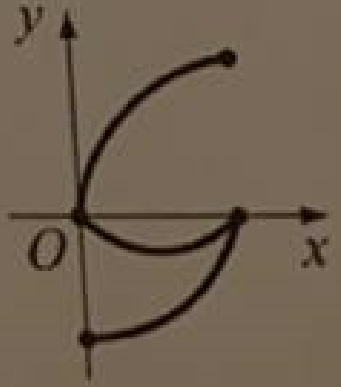
\includegraphics[scale=0.35]{graf930.png}}
\end{figure}\\
(А) $f(x)+g(x);$\\
(Б) $f(x)-g(x);$\\
(В) $f(x)\cdot g(x);$\\
(Г) $\cfrac{f(x)}{g(x)};$\\
(Д) $-f(x)\cdot g(x);$\\
81. Определите, при каких значениях параметра $a$ уравнение $(\sqrt{x}-2)(ax+2)(3x-2a)=0$ имеет ровно 2 различных корня.\\
82. а) Решите графически неравенство $\sqrt{x+3}>1+x;$\\
б) Сколько решений в зависимости от  $a$ имеет уравнение $\sqrt{x+3}=1+ax?$\\
83. Найдите все значения, которые принимает выражение $x+y,$ если $|y|=x(2-x).$\\
84. Найдите наименьшее значение суммы квадратов корней уравнения $x^2+3x+a=0$ и значение $a,$ при котором оно достигается.\\
85. Известно, что сумма квадратов корней уравнения $x^2-2x + q = 0$ равна 10084.
Найдите корни уравнения и значение $q.$\\
86. Известно, что сумма квадратов корней уравнения $x^2 -3x + q = 0$ равна 2249.
Найдите корни уравнения и $q.$\\
87. $f(x)=\sqrt{x^2+10x+34}+x-3.$ Найти координаты всех точек графика заданной функции,
равноудалённых от осей координат.\\
88. $f(x)=\sqrt{x^2+4x+8}-x-2.$ Найти координаты всех точек графика заданной функции,
равноудалённых от осей координат.\\
89. Прямая проходит через точку с координатами (10;0) и пересекает параболу $y=x^2$ в точках с абсциссами $x_1$ и $x_2.$ Найдите $\cfrac{1}{x_1}+\cfrac{1}{x_2}.$\\
90. Квадратный трёхчлен $f(x)=x^2+ax+b$ имеет два корня, один из которых лежит внутри отрезка  $[0;1],$ а
другой --- вне этого отрезка. Определите знак $f(b).$\\
91. Найдите целое число  $a,$ при котором выражение  $(x-a)(x-10)+1$ раскладывается в произведение $(x+b)(x+c)$ с целыми  $b$ и  $c.$\\
92. Известно, что $f(2x)=\cfrac{x+1}{2x+3}.$ Найдите корни уравнения $f(x)-1=0.$\\
93. При каком значении $a$ выражение $x^2+\cfrac{a^2}{x^2}-4\left(x+\cfrac{a}{x}\right)+10$ является полным квадратом?\\
94. При каких значениях параметра $a$ произведение корней уравнения $\cfrac{3x}{x^2+5x+9}=a$ равно 9?
\newpage
